\documentclass{standalone}
\usepackage{tikz}
\usetikzlibrary{patterns, positioning}

\begin{document}
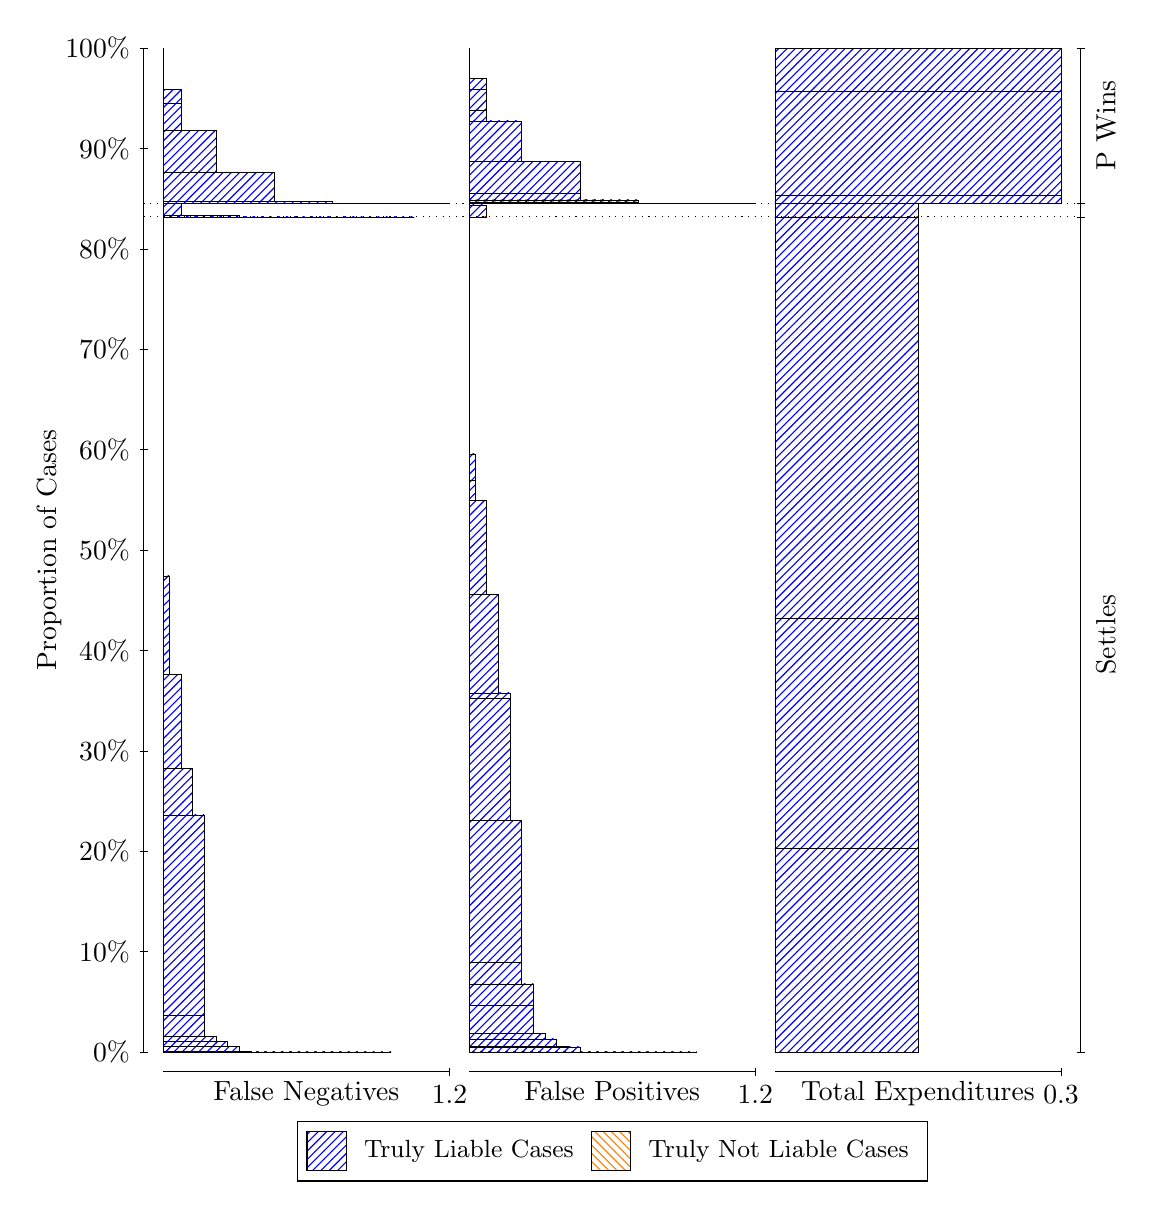
\begin{tikzpicture}
\draw[black, very thin] (1.5,1.75) -- (1.5,14.5);
\node[rotate=90, anchor=center] at (0.3, 8.125) {Proportion of Cases};
\draw[black, very thin] (1.45,1.75) -- (1.55,1.75);
\node[anchor=east] at (1.45, 1.75) {0\%};
\draw[black, very thin] (1.45,3.025) -- (1.55,3.025);
\node[anchor=east] at (1.45, 3.025) {10\%};
\draw[black, very thin] (1.45,4.3) -- (1.55,4.3);
\node[anchor=east] at (1.45, 4.3) {20\%};
\draw[black, very thin] (1.45,5.575) -- (1.55,5.575);
\node[anchor=east] at (1.45, 5.575) {30\%};
\draw[black, very thin] (1.45,6.85) -- (1.55,6.85);
\node[anchor=east] at (1.45, 6.85) {40\%};
\draw[black, very thin] (1.45,8.125) -- (1.55,8.125);
\node[anchor=east] at (1.45, 8.125) {50\%};
\draw[black, very thin] (1.45,9.4) -- (1.55,9.4);
\node[anchor=east] at (1.45, 9.4) {60\%};
\draw[black, very thin] (1.45,10.675) -- (1.55,10.675);
\node[anchor=east] at (1.45, 10.675) {70\%};
\draw[black, very thin] (1.45,11.95) -- (1.55,11.95);
\node[anchor=east] at (1.45, 11.95) {80\%};
\draw[black, very thin] (1.45,13.225) -- (1.55,13.225);
\node[anchor=east] at (1.45, 13.225) {90\%};
\draw[black, very thin] (1.45,14.5) -- (1.55,14.5);
\node[anchor=east] at (1.45, 14.5) {100\%};

\draw[black, very thin] (13.4,1.75) -- (13.4,14.5);
\draw[black, very thin] (13.35,1.75) -- (13.45,1.75);
\node[anchor=west] at (13.35, 1.75) {};
\draw[black, very thin] (13.35,12.355) -- (13.45,12.355);
\node[anchor=west] at (13.35, 12.355) {};
\draw[black, very thin] (13.35,12.531) -- (13.45,12.531);
\node[anchor=west] at (13.35, 12.531) {};
\draw[black, very thin] (13.35,14.5) -- (13.45,14.5);
\node[anchor=west] at (13.35, 14.5) {};

\draw[black, very thin, pattern color=blue, pattern=north east lines] (1.75,1.75) rectangle (4.6418,1.75);
\draw[black, very thin, pattern color=blue, pattern=north east lines] (1.75,1.75) rectangle (4.3452,1.75);
\draw[black, very thin, pattern color=blue, pattern=north east lines] (1.75,1.75) rectangle (4.0486,1.75);
\draw[black, very thin, pattern color=blue, pattern=north east lines] (1.75,1.75) rectangle (3.9003,1.75);
\draw[black, very thin, pattern color=blue, pattern=north east lines] (1.75,1.75) rectangle (3.752,1.75);
\draw[black, very thin, pattern color=blue, pattern=north east lines] (1.75,1.75) rectangle (3.6037,1.75);
\draw[black, very thin, pattern color=blue, pattern=north east lines] (1.75,1.75) rectangle (3.4554,1.75);
\draw[black, very thin, pattern color=blue, pattern=north east lines] (1.75,1.75) rectangle (3.3071,1.75);
\draw[black, very thin, pattern color=blue, pattern=north east lines] (1.75,1.75) rectangle (3.1588,1.75);
\draw[black, very thin, pattern color=blue, pattern=north east lines] (1.75,1.75) rectangle (3.0105,1.7506);
\draw[black, very thin, pattern color=blue, pattern=north east lines] (1.75,1.7506) rectangle (2.8622,1.7551);
\draw[black, very thin, pattern color=blue, pattern=north east lines] (1.75,1.7551) rectangle (2.7139,1.8184);
\draw[black, very thin, pattern color=blue, pattern=north east lines] (1.75,1.8184) rectangle (2.5656,1.8837);
\draw[black, very thin, pattern color=blue, pattern=north east lines] (1.75,1.8837) rectangle (2.5656,1.8837);
\draw[black, very thin, pattern color=blue, pattern=north east lines] (1.75,1.8837) rectangle (2.4173,1.945);
\draw[black, very thin, pattern color=blue, pattern=north east lines] (1.75,1.945) rectangle (2.269,2.2189);
\draw[black, very thin, pattern color=blue, pattern=north east lines] (1.75,2.2189) rectangle (2.269,4.7607);
\draw[black, very thin, pattern color=blue, pattern=north east lines] (1.75,4.7607) rectangle (2.1207,5.3521);
\draw[black, very thin, pattern color=blue, pattern=north east lines] (1.75,5.3521) rectangle (1.9724,6.5412);
\draw[black, very thin, pattern color=blue, pattern=north east lines] (1.75,6.5412) rectangle (1.8241,7.7959);
\draw[black, very thin, pattern color=blue, pattern=north east lines] (1.75,7.7959) rectangle (1.8241,7.7959);
\draw[black, very thin, pattern color=orange, pattern=north west lines] (1.75,7.7959) rectangle (1.75,7.7959);
\draw[black, very thin, pattern color=blue, pattern=north east lines] (1.75,7.7959) rectangle (1.75,12.355);
\draw[black, very thin, pattern color=blue, pattern=north east lines] (1.75,12.355) rectangle (4.9384,12.355);
\draw[black, very thin, pattern color=blue, pattern=north east lines] (1.75,12.355) rectangle (4.1969,12.355);
\draw[black, very thin, pattern color=blue, pattern=north east lines] (1.75,12.355) rectangle (3.4554,12.355);
\draw[black, very thin, pattern color=blue, pattern=north east lines] (1.75,12.355) rectangle (2.7139,12.379);
\draw[black, very thin, pattern color=blue, pattern=north east lines] (1.75,12.379) rectangle (1.9724,12.531);
\draw[black, very thin, pattern color=orange, pattern=north west lines] (1.75,12.531) rectangle (1.75,12.531);
\draw[black, very thin, pattern color=blue, pattern=north east lines] (1.75,12.531) rectangle (5.3833,12.531);
\draw[black, very thin, pattern color=blue, pattern=north east lines] (1.75,12.531) rectangle (4.6418,12.531);
\draw[black, very thin, pattern color=blue, pattern=north east lines] (1.75,12.531) rectangle (4.1969,12.531);
\draw[black, very thin, pattern color=blue, pattern=north east lines] (1.75,12.531) rectangle (3.9003,12.553);
\draw[black, very thin, pattern color=blue, pattern=north east lines] (1.75,12.553) rectangle (3.4554,12.553);
\draw[black, very thin, pattern color=blue, pattern=north east lines] (1.75,12.553) rectangle (3.1588,12.918);
\draw[black, very thin, pattern color=blue, pattern=north east lines] (1.75,12.918) rectangle (2.7139,12.919);
\draw[black, very thin, pattern color=blue, pattern=north east lines] (1.75,12.919) rectangle (2.7139,12.921);
\draw[black, very thin, pattern color=blue, pattern=north east lines] (1.75,12.921) rectangle (2.4173,13.457);
\draw[black, very thin, pattern color=blue, pattern=north east lines] (1.75,13.457) rectangle (1.9724,13.797);
\draw[black, very thin, pattern color=blue, pattern=north east lines] (1.75,13.797) rectangle (1.9724,13.973);
\draw[black, very thin, pattern color=orange, pattern=north west lines] (1.75,13.973) rectangle (1.75,13.973);
\draw[black, very thin, pattern color=blue, pattern=north east lines] (1.75,13.973) rectangle (1.75,14.5);
\draw[black, very thin, pattern color=orange, pattern=north west lines] (5.6333,1.75) rectangle (8.5252,1.75);
\draw[black, very thin, pattern color=blue, pattern=north east lines] (5.6333,1.75) rectangle (8.5252,1.75);
\draw[black, very thin, pattern color=orange, pattern=north west lines] (5.6333,1.75) rectangle (8.2286,1.75);
\draw[black, very thin, pattern color=blue, pattern=north east lines] (5.6333,1.75) rectangle (8.2286,1.75);
\draw[black, very thin, pattern color=orange, pattern=north west lines] (5.6333,1.75) rectangle (7.932,1.75);
\draw[black, very thin, pattern color=blue, pattern=north east lines] (5.6333,1.75) rectangle (7.932,1.75);
\draw[black, very thin, pattern color=blue, pattern=north east lines] (5.6333,1.75) rectangle (7.7837,1.75);
\draw[black, very thin, pattern color=orange, pattern=north west lines] (5.6333,1.75) rectangle (7.6354,1.75);
\draw[black, very thin, pattern color=blue, pattern=north east lines] (5.6333,1.75) rectangle (7.6354,1.75);
\draw[black, very thin, pattern color=blue, pattern=north east lines] (5.6333,1.75) rectangle (7.4871,1.75);
\draw[black, very thin, pattern color=orange, pattern=north west lines] (5.6333,1.75) rectangle (7.3388,1.75);
\draw[black, very thin, pattern color=blue, pattern=north east lines] (5.6333,1.75) rectangle (7.3388,1.7501);
\draw[black, very thin, pattern color=blue, pattern=north east lines] (5.6333,1.7501) rectangle (7.1905,1.7506);
\draw[black, very thin, pattern color=orange, pattern=north west lines] (5.6333,1.7506) rectangle (7.0422,1.7506);
\draw[black, very thin, pattern color=blue, pattern=north east lines] (5.6333,1.7506) rectangle (7.0422,1.7515);
\draw[black, very thin, pattern color=blue, pattern=north east lines] (5.6333,1.7515) rectangle (7.0422,1.8157);
\draw[black, very thin, pattern color=blue, pattern=north east lines] (5.6333,1.8157) rectangle (6.8939,1.818);
\draw[black, very thin, pattern color=orange, pattern=north west lines] (5.6333,1.818) rectangle (6.7456,1.818);
\draw[black, very thin, pattern color=blue, pattern=north east lines] (5.6333,1.818) rectangle (6.7456,1.9168);
\draw[black, very thin, pattern color=blue, pattern=north east lines] (5.6333,1.9168) rectangle (6.5973,1.9817);
\draw[black, very thin, pattern color=orange, pattern=north west lines] (5.6333,1.9817) rectangle (6.449,1.9817);
\draw[black, very thin, pattern color=blue, pattern=north east lines] (5.6333,1.9817) rectangle (6.449,2.339);
\draw[black, very thin, pattern color=blue, pattern=north east lines] (5.6333,2.339) rectangle (6.449,2.6152);
\draw[black, very thin, pattern color=blue, pattern=north east lines] (5.6333,2.6152) rectangle (6.3007,2.8908);
\draw[black, very thin, pattern color=blue, pattern=north east lines] (5.6333,2.8908) rectangle (6.3007,4.6949);
\draw[black, very thin, pattern color=orange, pattern=north west lines] (5.6333,4.6949) rectangle (6.1524,4.6949);
\draw[black, very thin, pattern color=blue, pattern=north east lines] (5.6333,4.6949) rectangle (6.1524,6.2454);
\draw[black, very thin, pattern color=blue, pattern=north east lines] (5.6333,6.2454) rectangle (6.1524,6.3091);
\draw[black, very thin, pattern color=blue, pattern=north east lines] (5.6333,6.3091) rectangle (6.0041,7.5638);
\draw[black, very thin, pattern color=blue, pattern=north east lines] (5.6333,7.5638) rectangle (5.8558,8.7529);
\draw[black, very thin, pattern color=blue, pattern=north east lines] (5.6333,8.7529) rectangle (5.7075,9.0064);
\draw[black, very thin, pattern color=blue, pattern=north east lines] (5.6333,9.0064) rectangle (5.7075,9.3443);
\draw[black, very thin, pattern color=blue, pattern=north east lines] (5.6333,9.3443) rectangle (5.6333,12.355);
\draw[black, very thin, pattern color=orange, pattern=north west lines] (5.6333,12.355) rectangle (5.8558,12.355);
\draw[black, very thin, pattern color=blue, pattern=north east lines] (5.6333,12.355) rectangle (5.8558,12.507);
\draw[black, very thin, pattern color=blue, pattern=north east lines] (5.6333,12.507) rectangle (5.6333,12.531);
\draw[black, very thin, pattern color=orange, pattern=north west lines] (5.6333,12.531) rectangle (9.2667,12.531);
\draw[black, very thin, pattern color=blue, pattern=north east lines] (5.6333,12.531) rectangle (9.2667,12.531);
\draw[black, very thin, pattern color=blue, pattern=north east lines] (5.6333,12.531) rectangle (8.5252,12.531);
\draw[black, very thin, pattern color=orange, pattern=north west lines] (5.6333,12.531) rectangle (8.5252,12.531);
\draw[black, very thin, pattern color=blue, pattern=north east lines] (5.6333,12.531) rectangle (8.5252,12.531);
\draw[black, very thin, pattern color=blue, pattern=north east lines] (5.6333,12.531) rectangle (7.7837,12.545);
\draw[black, very thin, pattern color=orange, pattern=north west lines] (5.6333,12.545) rectangle (7.7837,12.545);
\draw[black, very thin, pattern color=blue, pattern=north east lines] (5.6333,12.545) rectangle (7.7837,12.571);
\draw[black, very thin, pattern color=orange, pattern=north west lines] (5.6333,12.571) rectangle (7.3388,12.571);
\draw[black, very thin, pattern color=blue, pattern=north east lines] (5.6333,12.571) rectangle (7.3388,12.571);
\draw[black, very thin, pattern color=blue, pattern=north east lines] (5.6333,12.571) rectangle (7.0422,12.651);
\draw[black, very thin, pattern color=orange, pattern=north west lines] (5.6333,12.651) rectangle (7.0422,12.651);
\draw[black, very thin, pattern color=blue, pattern=north east lines] (5.6333,12.651) rectangle (7.0422,13.057);
\draw[black, very thin, pattern color=orange, pattern=north west lines] (5.6333,13.057) rectangle (6.5973,13.057);
\draw[black, very thin, pattern color=blue, pattern=north east lines] (5.6333,13.057) rectangle (6.5973,13.058);
\draw[black, very thin, pattern color=blue, pattern=north east lines] (5.6333,13.058) rectangle (6.5973,13.058);
\draw[black, very thin, pattern color=blue, pattern=north east lines] (5.6333,13.058) rectangle (6.3007,13.06);
\draw[black, very thin, pattern color=blue, pattern=north east lines] (5.6333,13.06) rectangle (6.3007,13.574);
\draw[black, very thin, pattern color=blue, pattern=north east lines] (5.6333,13.574) rectangle (5.8558,13.714);
\draw[black, very thin, pattern color=orange, pattern=north west lines] (5.6333,13.714) rectangle (5.8558,13.714);
\draw[black, very thin, pattern color=blue, pattern=north east lines] (5.6333,13.714) rectangle (5.8558,13.973);
\draw[black, very thin, pattern color=blue, pattern=north east lines] (5.6333,13.973) rectangle (5.8558,14.11);
\draw[black, very thin, pattern color=blue, pattern=north east lines] (5.6333,14.11) rectangle (5.6333,14.5);
\draw[black, very thin, pattern color=orange, pattern=north west lines] (9.5167,1.75) rectangle (11.333,1.75);
\draw[black, very thin, pattern color=blue, pattern=north east lines] (9.5167,1.75) rectangle (11.333,4.331);
\draw[black, very thin, pattern color=orange, pattern=north west lines] (9.5167,4.331) rectangle (11.333,4.331);
\draw[black, very thin, pattern color=blue, pattern=north east lines] (9.5167,4.331) rectangle (11.333,7.2572);
\draw[black, very thin, pattern color=orange, pattern=north west lines] (9.5167,7.2572) rectangle (11.333,7.2572);
\draw[black, very thin, pattern color=blue, pattern=north east lines] (9.5167,7.2572) rectangle (11.333,12.355);
\draw[black, very thin, pattern color=orange, pattern=north west lines] (9.5167,12.355) rectangle (11.333,12.355);
\draw[black, very thin, pattern color=blue, pattern=north east lines] (9.5167,12.355) rectangle (11.333,12.531);
\draw[black, very thin, pattern color=orange, pattern=north west lines] (9.5167,12.531) rectangle (13.15,12.531);
\draw[black, very thin, pattern color=blue, pattern=north east lines] (9.5167,12.531) rectangle (13.15,12.628);
\draw[black, very thin, pattern color=orange, pattern=north west lines] (9.5167,12.628) rectangle (13.15,12.628);
\draw[black, very thin, pattern color=blue, pattern=north east lines] (9.5167,12.628) rectangle (13.15,13.953);
\draw[black, very thin, pattern color=orange, pattern=north west lines] (9.5167,13.953) rectangle (13.15,13.953);
\draw[black, very thin, pattern color=blue, pattern=north east lines] (9.5167,13.953) rectangle (13.15,14.5);
\draw[black, dotted] (1.5,12.355) -- (13.4,12.355);
\draw[black, dotted] (1.5,12.531) -- (13.4,12.531);
\draw[black, very thin] (1.75,1.5) -- (5.3833,1.5);
\node[anchor=north] at (3.5667, 1.5) {False Negatives};
\draw[black, very thin] (5.3833,1.45) -- (5.3833,1.55);
\node[anchor=north] at (5.3833, 1.45) {1.2};

\draw[black, very thin] (5.6333,1.5) -- (9.2667,1.5);
\node[anchor=north] at (7.45, 1.5) {False Positives};
\draw[black, very thin] (9.2667,1.45) -- (9.2667,1.55);
\node[anchor=north] at (9.2667, 1.45) {1.2};

\draw[black, very thin] (9.5167,1.5) -- (13.15,1.5);
\node[anchor=north] at (11.333, 1.5) {Total Expenditures};
\draw[black, very thin] (13.15,1.45) -- (13.15,1.55);
\node[anchor=north] at (13.15, 1.45) {0.3};

\node[black, centered, rotate=90] at (13.72, 7.0525) {Settles};

\node[black, centered, rotate=90] at (13.72, 13.515) {P Wins};

\draw (7.449999999999999,1.5) node[draw=none] (baseCoordinate) {};
\begin{scope}[align=center]
        \matrix[scale=0.5, draw=black, below=0.5cm of baseCoordinate, nodes={draw}, column sep=0.1cm]{
            \node[rectangle, draw, minimum width=0.5cm, minimum height=0.5cm, pattern=north east lines, pattern color=blue] {}; &
            \node[draw=none, font=\small] (B) {Truly Liable Cases}; &
            \node[rectangle, draw, minimum width=0.5cm, minimum height=0.5cm, pattern=north west lines, pattern color=orange] {}; &
            \node[draw=none, font=\small] (B) {Truly Not Liable Cases}; \\
            };
\end{scope}

\end{tikzpicture}
\end{document}